\begin{question}
\noindent In a Valorant map-design tool, a designer places a triangular "spike site" marker $T$ on a coordinate grid, with vertices $A(1,1)$, $B(1,3)$ and $C(3,1)$.

The designer first reflects $T$ in the line $y = x$ to get triangle $T_1$. She then reflects $T_1$ in the $x$-axis to get triangle $T_2$, as shown on the grid below.

\begin{center}
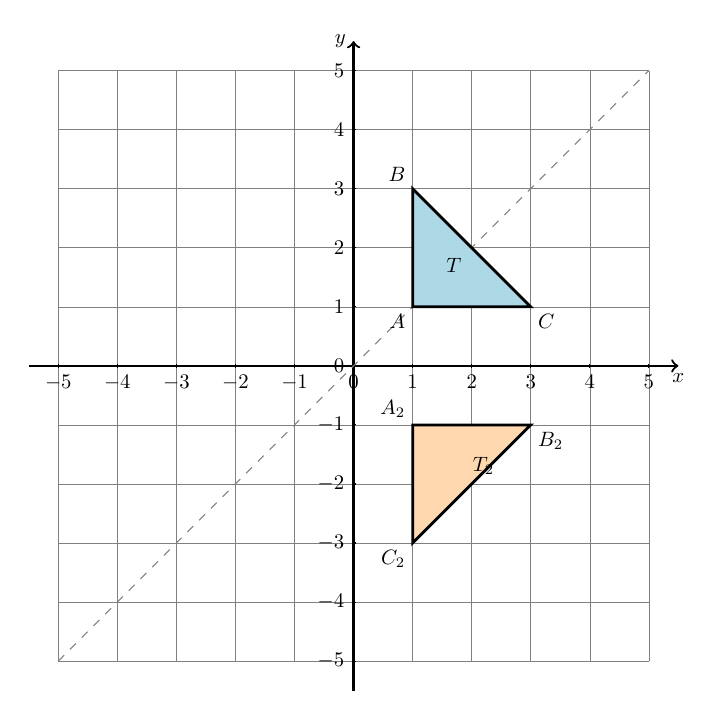
\begin{tikzpicture}[scale=0.75, transform shape]
    \def\axisLimit{5}
    \definecolor{borderColour}{HTML}{000000}
    \definecolor{fillColourT}{HTML}{ADD8E6}
    \definecolor{fillColourT2}{HTML}{FFD8B0}

    % Draw grid
    \draw[step=1cm,gray,very thin] (-\axisLimit,-\axisLimit) grid (\axisLimit,\axisLimit);

    % Draw axes
    \draw[thick,->] (-\axisLimit-0.5,0) -- (\axisLimit+0.5,0) node[anchor=north] {$x$};
    \draw[thick,->] (0,-\axisLimit-0.5) -- (0,\axisLimit+0.5) node[anchor=east] {$y$};

    % Label x-axis and y-axis
    \foreach \x in {-\axisLimit,...,\axisLimit}
        \draw (\x cm,1pt) -- (\x cm,-1pt) node[anchor=north] {$\x$};
    \foreach \y in {-\axisLimit,...,\axisLimit}
        \draw (1pt,\y cm) -- (-1pt,\y cm) node[anchor=east] {$\y$};

    % Line y = x for reference
    \draw[dashed, gray] (-\axisLimit,-\axisLimit) -- (\axisLimit,\axisLimit);

    % Triangle T: A(1,1), B(1,3), C(3,1)
    \coordinate (A) at (1,1);
    \coordinate (B) at (1,3);
    \coordinate (C) at (3,1);
    \filldraw[fill=fillColourT, draw=borderColour, line width=1pt] (A) -- (B) -- (C) -- cycle;
    \node[below left] at (A) {$A$};
    \node[above left] at (B) {$B$};
    \node[below right] at (C) {$C$};
    \node at (1.7,1.7) {$T$};

    % Triangle T2: after reflecting in y=x then in x-axis
    % T1 (reflect in y=x): A1(1,1), B1(3,1), C1(1,3)
    % T2 (reflect in x-axis): A2(1,-1), B2(3,-1), C2(1,-3)
    \coordinate (A2) at (1,-1);
    \coordinate (B2) at (3,-1);
    \coordinate (C2) at (1,-3);
    \filldraw[fill=fillColourT2, draw=borderColour, line width=1pt] (A2) -- (B2) -- (C2) -- cycle;
    \node[above left] at (A2) {$A_2$};
    \node[below right] at (B2) {$B_2$};
    \node[below left] at (C2) {$C_2$};
    \node at (2.2,-1.7) {$T_2$};

\end{tikzpicture}
\end{center}

\noindent (a) Find the coordinates of the vertices of $T_1$ (the image of $T$ after reflecting in the line $y = x$), and hence the coordinates of the vertices of $T_2$ (the image of $T_1$ after reflecting in the $x$-axis).

\vspace{3cm}
\answermarks{2}

\noindent (b) By comparing the coordinates of $T$ and $T_2$, show that the combined transformation (reflection in $y = x$ followed by reflection in the $x$-axis) is equivalent to a single rotation, stating the angle, direction and centre of this rotation.

\vspace{4cm}
\answermarks{2}

\end{question}